%%%%%%%%%%%%%%%%%%%%%%%%%%%%%%%%
% Section 5. Application: DAPO with RSP
%%%%%%%%%%%%%%%%%%%%%%%%%%%%%%%%

\section{Application: RSP를 이용한 DAPO 학습}\label{sec:application}

지금까지의 실험 분석은 RSP를 추론 시점에서만 평가했다. \S\ref{sec:multipath}는 독립 RSP 추첨이 rollout 다양성에 의존하는 모든 sampling 기반 최적화에 도움이 될 것이라고 예측한다. 이를 검증하기 위해 RSP를 GRPO 기반 RL 학습 파이프라인에 통합한다. 구현 세부와 step별 결과는 Appendix~\ref{app:dapo}에 있다.

\paragraph{DAPO.}
DAPO \citep{yu2025dapo}는 GRPO \citep{shao2024deepseekmath}의 손실 항을 수정해 긴 chain-of-thought RL 학습 동안 rollout 다양성을 손실 단에서 유지한다. 반면 RSP는 손실 계산 전에 rollout 분포 자체에 섭동을 주어 \emph{입력 단}에서 다양성을 유발한다(\S\ref{sec:diversity}). 두 다양성 원천이 결합해 추가 이득을 만들 수 있는지 검증하기 위해 DAPO를 testbed로 쓴다. $i$번째 rollout 응답을 $o_i$, 중요도 비를 $r_{i,t}(\theta) = \pi_\theta(o_{i,t}\mid q, [\mathbf{H}_g,] o_{i,<t}) / \pi_{\theta_{\text{old}}}(o_{i,t}\mid q, [\mathbf{H}_g,] o_{i,<t})$, 그룹 상대 advantage를 $\hat{A}_{i,t}$, 비대칭 clip 범위를 $(\varepsilon_{\text{low}}, \varepsilon_{\text{high}})$, prompt에 결합한 RSP를 $\mathbf{H}_g$라 하면 DAPO + RSP의 목적함수는
\begin{equation}\label{eq:dapo_rsp}
\mathcal{J}_{\text{DAPO+RSP}}(\theta)
\;=\;
\mathbb{E}\!\left[
\frac{1}{\sum_i |o_i|}
\sum_{i,t}
\min\!\Big(r_{i,t}\hat{A}_{i,t},\,
\text{clip}\big(r_{i,t},\,1{-}\varepsilon_{\text{low}},\,1{+}\varepsilon_{\text{high}}\big)\hat{A}_{i,t}\Big)
\right].
\end{equation}

\paragraph{설정.}
Qwen2.5-Math-7B를 MATH Level-3--5 subset(약 8{,}500 prompt)에서 SimpleRL-Zoo \citep{zeng2025simplerl} 파이프라인과 Eq.~\eqref{eq:dapo_rsp}로 학습한다. 매 step은 prompt 1{,}024개 배치 위에서 $\tau{=}1.0$, $G=8$ rollout, 총 100 step(약 12 epoch). \emph{DAPO}와 \emph{DAPO + RSP}를 비교하며, 후자는 rollout에만 suffix RSP($L=20$)를 적용하고 평가는 RSP 없이 수행한다. 평가는 7개 수학 추론 벤치마크(MATH-500 \citep{lightman2024lets}, AIME 2024, AMC 2023, GSM8K \citep{cobbe2021training}, GaoKao 2023-EN, OlympiadBench \citep{he2024olympiad}, Minerva Math \citep{lewkowycz2022minerva})에서 진행한다. 작은 경시대회 셋(AIME 2024, AMC 2023)은 분산 축소를 위해 $\tau{=}1.0$에서 Avg@32, 큰 셋은 greedy 단일 샘플로 채점한다. 보고는 두 방법이 peak에서 다른 4-벤치마크(MATH-500, AIME 2024, GSM8K, Minerva Math)의 가중치 없는 평균이며, 나머지 셋은 동률이다.

\paragraph{결과.}
Figure~\ref{fig:dapo_curve}는 학습 step에 따른 평균 정확도, Table~\ref{tab:dapo_peak}은 각 방법의 peak step 벤치마크별 정확도다.

\begin{table}[!ht]
\centering
\caption{Qwen2.5-Math-7B에서 각 방법의 peak step 벤치마크별 정확도(\%). \textbf{굵게}는 두 RL 방법 중 더 높은 쪽이고, Avg는 가중치 없는 4-벤치마크 평균이다.}
\label{tab:dapo_peak}
\footnotesize
\setlength{\tabcolsep}{6pt}
\renewcommand{\arraystretch}{0.9}
\begin{tabular}{l cccc c}
\toprule
\textbf{Method} & \textbf{GSM8K} & \textbf{MATH-500} & \textbf{Minerva} & \textbf{AIME 24} & \textbf{Avg} \\
\midrule
Base                & 57.2 & 52.6 & 13.6 & 8.6  & 33.00 \\
DAPO                & 86.3 & 78.2 & 37.5 & 22.6 & 56.15 \\
\rowcolor{blue!10}
DAPO~+~RSP          & \textbf{87.7} & \textbf{78.6} & \textbf{39.7} & \textbf{23.6} & \textbf{57.40} \\
\bottomrule
\end{tabular}
\end{table}

\paragraph{해석.}
\begin{wrapfigure}{r}{0.42\textwidth}
  \vspace{-1.0em}
  \centering
  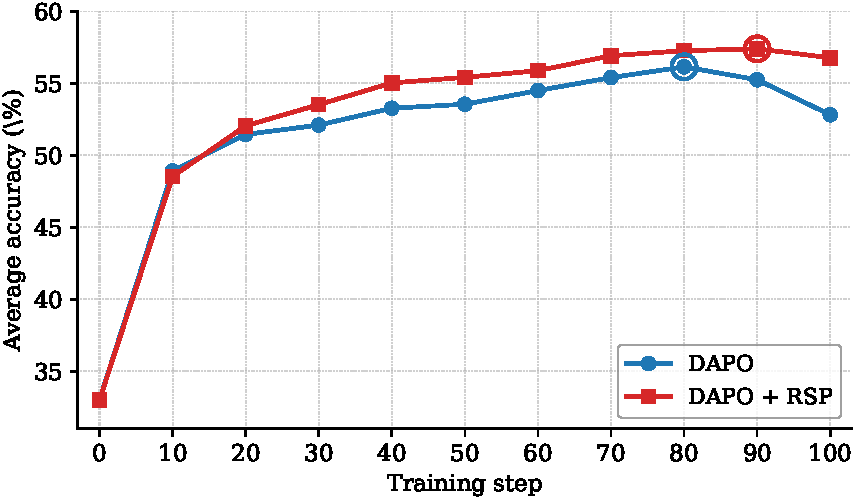
\includegraphics[width=0.40\textwidth]{img/dapo/dapo_avg_curve.pdf}
  \caption{Qwen2.5-Math-7B의 4-벤치마크 평균 정확도. DAPO~+~RSP는 step 90에서 peak에 도달해 step 100까지 안정적으로 유지되는 반면, DAPO는 step 80 이후 감소한다.}
  \label{fig:dapo_curve}
\end{wrapfigure}
DAPO 단독은 step 80 peak(56.15\%) 후 step 100에서 52.82\%로 떨어지지만, DAPO~+~RSP는 step 90 peak 57.40\%까지 상승해 step 100에서도 56.78\%를 유지한다(+1.25\,pp peak 상승). 입력 공간 재추첨이 DAPO의 손실 단 entropy 관리와 \emph{상보적} 다양성 원천이라는 점과 일치한다 — RSP는 rollout 사이 독립 섭동을 주입해 policy entropy에 의존하지 않는다. 초반엔 reward 성장이 느리지만(두 곡선 step 20 교차) 결국 붕괴 지연과 peak 상승으로 누적되며, 이는 RL exploration--exploitation 패턴 \citep{sutton2018reinforcement}과 정합한다. 한계와 견고성 점검은 Appendix~\ref{app:dapo_limitations}에 있다.
